% Copyright 2024 Kieran W Harvie. All rights reserved.

\section{Bernstein Basis Polynomials}
The $k^\text{th}$ Bernstein basis polynomial of order $n$ is defined as:
\[
	b_{k,n}(t) = \binom{n}{k}(1-t)^{n-k}t^k
\]
Where we follow that convention that $\binom{n}{k}=0$ when $k<0$ or $k>n$.
\\

They have some really useful properties that lend them themselves to applications like
approximating continuous functions,
numerically stable polynomial evaluation, 
and are the foundation of Bézier geometry.
To this end it will be useful to collect some of those properties bellow.
\begin{center}
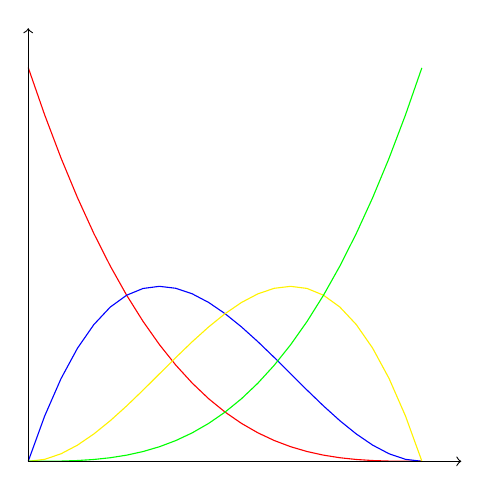
\begin{tikzpicture}[domain=0:1,scale=5]
	\draw[red] plot (\x,{(1-\x)^3});
	\draw[blue] plot(\x,{3*\x*(1-\x)^2});
	\draw[yellow] plot (\x,{3*\x*\x*(1-\x)});
	\draw[green] plot (\x,{\x*\x*\x});

	\draw[<->] (0,1.1)--(0,0)--(1.1,0);
\end{tikzpicture}

The four Bernstein basis polynomials of degree three over $[0,1]$.
\end{center}

\subsubsection{Fundamental Recursion:}
The most fundamental property of Bernstein basis polynomials is the recursion:
\[b_{k,n+1}(t) = (1-t)b_{k,n}(t)+tb_{k-1,n}(t)\]
And that there are $n+1$ polynomials of order $n$,
since when $k<0$ or $k>n$ we have:
\[b_{k,n}(t) = 0\]
Both of these properties can be verified by inspection of the definition and let us create a table of low order Bernstein basis polynomials to further cultivate intuition:
\[
\begin{array}{|c|ccccc|}
	\hline
	b_{k,n}(t)&0&1&2&3&4\\
	\hline
	4&(1-t)^4&4t(1-t)^3&6t^2(1-t)^2&4t^3(1-t)&t^4\\
	3&(1-t)^3&3t(1-t)^2&3t^2(1-t)&t^3&\\
	2&(1-t)^2&2t(1-t)&t^2&&\\
	1&1-t&t&&&\\
	0&1&&&&\\
	\hline
\end{array}
\]

\subsubsection{Endpoints:}
In most application we will be considering $t\in[0,1]$.
So it makes sense to consider $b_{k,n}(0)$ and $b_{k,n}(1)$ as the `endpoints' and note  their values as:
\[b_{k,n}(0) = \begin{cases}1& k=0\\0&k\neq0\\\end{cases}\quad\text{and}\quad b_{k,n}(1) = \begin{cases}1& k= n\\0&k\neq n\\\end{cases}\]

\subsubsection{Inner Product and Partition of Unity:}
The following combinatorial identity can be verified by expansion:
\[\binom{n}{l}\binom{l}{k} = \binom{n}{k}\binom{n-k}{l-k}\]
When combined with the binomial theorem it allows us evaluate an `inner product' of Bernstein basis polynomials:
\[\begin{aligned}
	\sum_{l=k}^nb_{k,l}(t)b_{l,n}(\tau) =& \sum_{l=k}^n\binom{n}{l}\binom{l}{k}t^l\tau^k(1-t)^{n-l}(1-\tau)^{l-k}\\
	=& \binom{n}{k}(t\tau)^k\sum_{l=k}^n\binom{n-k}{l-k}(1-t)^{n-l}(t(1-\tau))^{l-k}\\
	=& \binom{n}{k}(t\tau)^k\sum_{l=0}^{n-k}\binom{n-k}{l}(1-t)^{n-l-k}(t(1-\tau))^{l}\\
	=& \binom{n}{k}(t\tau)^k(1-t+t(1-\tau))^{n-k}\\
	=& b_{k,n}(t\tau)\\
\end{aligned}\]
In particular,
when $k$ and $\tau$ equal $0$, we have:
\[b_{k,l}(\tau) = b_{k,n}(t\tau) = 1\]
Which substitution into the general case gives:
\[\sum_{l=0}^nb_{l,n}(t) = 1\]
Hence,
for any given $n$,
the polynomials $b_{k,n}(t)$ are a partition of unity.

\subsubsection{Reflection:}
From the following binomial formula:
\[\binom{n}{k}=\binom{n}{n-k}\]
We get the following formula for reflecting argument around $\frac{1}{2}$:
\[b_{k,n}(t) = b_{n-k,n}(1-t)\]
Which gives my favourite Bernstein basis polynomial formula: 
\[ b_{k,m}(\tau+(1-\tau)t) = \sum_{l=0}^kb_{k-l,n-l}(\tau)b_{l,n}(t) \]
By applying the reflection to the inner product formula:
\[\begin{aligned}
	b_{k,n}(\tau+(1-\tau)t) =& b_{k,n}(1-(1-t)(1-\tau))\\
	=& b_{n-k,n}((1-t)(1-\tau))\\
	=&\sum_{l=n-k}^nb_{n-k,l}(1-\tau)b_{l,n}(1-t)\\
	=&\sum_{l=n-k}^nb_{k-(n-l),l}(\tau)b_{n-l,n}(t)\\
\end{aligned}\]
And then change the summation order so $l$ goes down from $n$ instead of up from $n-k$.

\subsubsection{Bounds:}
When $t\in[0,1]$ we have both $t\geq0$ and $1-t\geq0$ and hence:
\[t\in [0,1] \Rightarrow b_{k,n}(t)\geq0 \]
Now since each individual polynomial is positive we have:
\[b_{k,n}(t) \leq \sum_{k=0}^nb_{k,n}(t) = 1\]

\subsubsection{Derivative:}
By direct application of the product rule we get:
\[b_{k,n+1}'(t) = k\binom{n+1}{k}(1-t)^{n+1-k}t^{k-1}-(n+1-k)\binom{n+1}{k}(1-t)^{n-k}t^k\]
Simpling the coefficients containing $k$ into the binomial coefficients we obtain:
\[b_{k,n+1}'(t) = (n+1)(b_{k-1,n}(t)-b_{k,n}(t))\]
If we instead factor common terms we get:
\[b_{k,n+1}'(t) = (1-t)^{n-k}t^{k-1}\binom{n+1}{k}\bigg(k(1-t)-(n+1-k)t\bigg)\]
When $t\in[0,1]$ the first three factors are non-negative,
hence there can only be an extrema where the fourth factor is zero at $t=\frac{k}{n+1}$.
By considering the endpoints this extrema must be a maximum and is the only extrema on $t\in[0,1]$.

\subsubsection{Useful Sums:}
We have already used binomial expansion when calculating the inner product.
However, if we consider the general expression:
\[(x+y)^n = \sum_{k=0}^n\binom{n}{k}x^{n-k}y^k\]	
When derived by $y$:
\[n(x+y)^{n-1} = \sum_{k=0}^nk\binom{n}{k}x^{n-k}y^{k-1}\]
Multiplied by $y(x+y)$:
\[ny(x+y)^n = (x+y)\sum_{k=0}^nk\binom{n}{k}x^{n-k}y^k\]
And having set $x=1-t$ and $y=t$:
\[nt = \sum_{k=0}^nk\binom{n}{k}(1-t)^{n-k}t^k\ = \sum_{k=0}^nkb_{k,n}(t)\]
We get this sum with simple terms.
The simplicity makes it a useful starting point and sanity check when writing algorithms involving the Bernstein basis polynomials.
For example,
if we are writing an algorithm for calculating the value of a Bernstein basis expansion at $t$ we know that if we choose linearly increasing coefficients we should get a linear function of $t$.
If we conversely want the Bernstein basis expansion of a linear function we know to use linearly increasing coefficients.	
\\

Through similar methods we get similar sums for higher powers, for example:
\[n(n-1)t^2 = \sum_{k=0}^nk(k-1)b_{k,n}(t)\]
They are useful for similar starting points and sanity checks for derivatives.
For example if we choose quadratically increasing coefficients in a Bernstein basis expansion we should get a linear derivative.
